\newpage

\section{Spilbeskrivelse}

Der udvikles et tekst-basseret spil kaldet "Dungeons and Gnoblins". Spillet består af fire dele en grafisk brugergrænseflade til interaktioner, en database til at gemme profiler og spil, en back-end til netværkskommunikation og selve spil logikken.

\subsection{Login-screen}
Det første brugeren bliver mødt af er en login-skærm. Her skal brugeren enten logge ind eller opretter en profil.  Herunder ses en illustration af spillets login-screen. 

\begin{figure}[H]
\centering
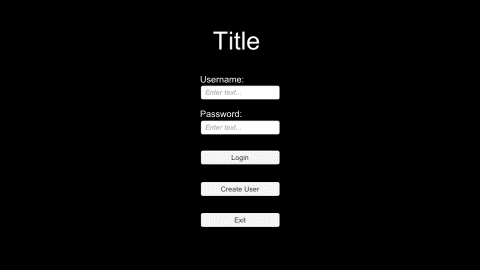
\includegraphics[width = \textwidth]{02-Body/Images/Loginscreen-udkast.png}
\caption{Udkast til loginscreen hvor man både kan logge ind på en eksisterende bruger og oprette en ny}
\label{fig:Loginscreen-udkast}
\end{figure}

\subsection{Core gameplay layout}
På \autoref{fig:Core-Gameplay-Layout-udkast} er vist en illustration af hvad brugeren møder ved indtrædelse i et rum. Til venstre ses en beskrivelse af rummet samt en liste af ting som er i rummet. Til højre ses et map af spillet, nedenfor dette er en række knapper som brugeren kan bruge til at interegere med spillet eksempelvis navigering eller opsamling af ting.


\begin{figure}[H]
\centering
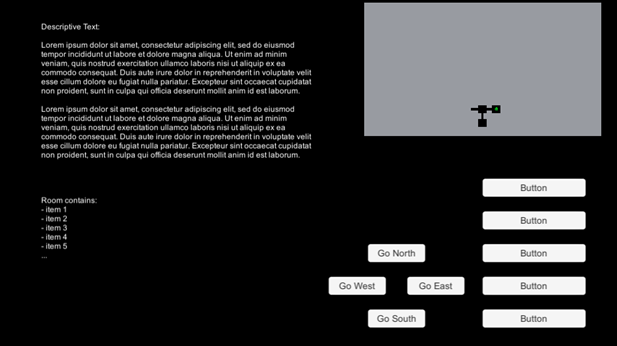
\includegraphics[width = \textwidth]{02-Body/Images/SpilLayout-udkast.png}
\caption{Udkast til core gameplay layout hvor man der til venstre en en beskrivelse af historien efterfulgt af ting man kan interagere med. I højre side er der øverst en visuel præsentation af spillets map og hvor spilleren er derpå. Nederst til højre kan man bevæge sig i spillet og der er knappet til at lave forskellige interaktioner.}
\label{fig:Core-Gameplay-Layout-udkast}
\end{figure}

Et rum kan indeholde fjender, som der kan kæmpes imod. En kamp foregår ved at spilleren og fjenden laver et "terninge kast", hvis der slåes højere end modstanderens "defense stats" gives skade til modstanderen. En spiller dør hvis denne mister alt sit liv og dermed er spillet tabt. På \autoref{fig:Combat-udkast} ses en illustration af combat screen.

\begin{figure}[H]
\centering
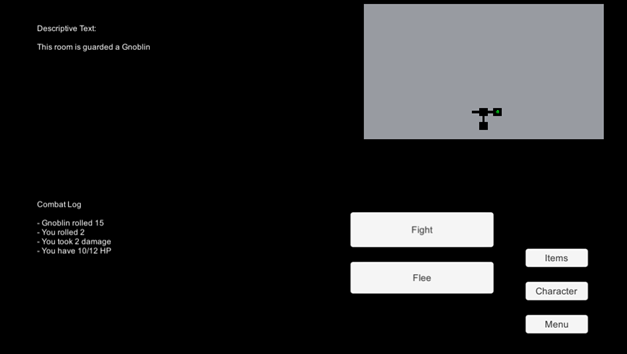
\includegraphics[width = \textwidth]{02-Body/Images/CombatScreen-udkast.png}
\caption{Udkast til combatscreen. Til venstre er der øverst en beskrivene tekst hvorunder der er en combatlog som beskriver fightens forløb. I højre side er der øverst en visuel præsentation af spillets map og hvor spilleren er derpå. Under mappet er der til venstre de to muligheder man har under en combat, fight og flee. Til højre for det, er der forskellige menu muligheder}
\label{fig:Combat-udkast}
\end{figure}

\subsection{Settings}
Det skal være muligt for spilleren at tilgå en menu med spillets indstillinger. Her kan spilleren ændre på resolution, window size og lydstyrken for spillet.

En illustration af hvordan denne menu kunne se ud er vist på \autoref{fig:Settings-udkast}.

\begin{figure}[H]
\centering
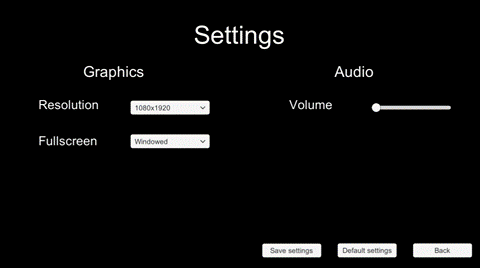
\includegraphics[width = \textwidth]{02-Body/Images/SettingsMenu-udkast.png}
\caption{Udkast til settings menuen, hvor man til venstre kan sætte spillets resolution og til højre kan sætte spillets musik volume.
Nederst er der 3 forskellige muligheder, gem settings, default settings og at gå tilbage}
\label{fig:Settings-udkast}
\end{figure}
